\chapter{The Standard Model of Particle Physics}

The standard model of particle physics is a quantum field
theory based on the gauge symmetry group
$\mathrm{SU(3)}_{\mathrm{C}}\times \mathrm{SU(2)}_{\mathrm{L}}\times
\mathrm{U(1)}_Y$. The corresponding gauge fields are
$\mathbf{G}_{\mu}$ (a $3\times3$ traceless Hermitian matrix),
$\mathbf{W}_{\mu}$ (a $2\times2$ traceless Hermitian matrix), and $B_{\mu}$,
respectively. The matter fields are chiral fermions, which fall into two
categories: quarks $u_R$, $u_L$, $d_R$, $d_L$ which transform in
the fundamental representation of $\mathrm{SU(3)}_{\mathrm{C}}$, and
leptons $e_R$, $e_L$, $\nu_R$, $\nu_L$, which are singlets of
$\mathrm{SU(3)}_{\mathrm{C}}$. All matter fields implicity have
three-component generation indices $e_i=(e,\mu,\tau),
\nu_i=(\nu_e,\nu_{\mu},\nu_{\tau}), u_i=(u,c,t),
d_i=(d,s,b)$. Eqn.~\ref{eqn:lsm} shows the standard model Langrangian
including mass terms.

{\footnotesize
\begin{tabular}{rcll}
$\mathcal{L}_{\mathrm{SM}}$ &$=$& $-\frac{1}{4}B_{\mu\nu}B^{\mu\nu} -
\frac{1}{8}\mathrm{tr}(\mathbf{W}_{\mu\nu}\mathbf{W}^{\mu\nu}) -
                                  \frac{1}{2}\mathrm{tr}(\mathbf{G}_{\mu\nu}\mathbf{G}^{\mu\nu})$
  & ($\mathrm{SU(3)}_{\mathrm{C}}\times \mathrm{SU(2)}_{\mathrm{L}}\times
\mathrm{U(1)}_Y$ gauge terms)\\
&& $(\bar\nu_L,\bar
   e_L)\tilde\sigma^{\mu}iD_{\mu}\displaystyle{\binom{\nu_L}{e_L}} +
   \bar e_R\sigma^{\mu}iD_{\mu}e_R + \bar v_R
   \sigma^{\mu}iD_{\mu}\nu_R + (\mathrm{h.c.})$& (lepton dynamical terms)\\
&& $(\bar u_L,\bar
   d_L)\tilde\sigma^{\mu}iD_{\mu}\displaystyle{\binom{u_L}{d_L}} +
   \bar u_R\sigma^{\mu}iD_{\mu}u_R + \bar d_R
   \sigma^{\mu}iD_{\mu}d_R + (\mathrm{h.c.})$& (quark dynamical
                                               terms)\\
&& $\bar{(D_{\mu}\phi)}D^{\mu}\phi - m_h^2[\bar\phi\phi -
   v^2/2]^2/2v^2$ &  (Higgs dynamical term and potential)
\end{tabular}
\begin{equation}
\label{eqn:lsm}
\end{equation}
}

Fig.~\ref{fig:standardmodel} shows the particles in the standard model
and Tab.~\ref{tab:representations} summarizes the
representations in which the fields transform under the standard model
gauge group.

\begin{figure}
\centering
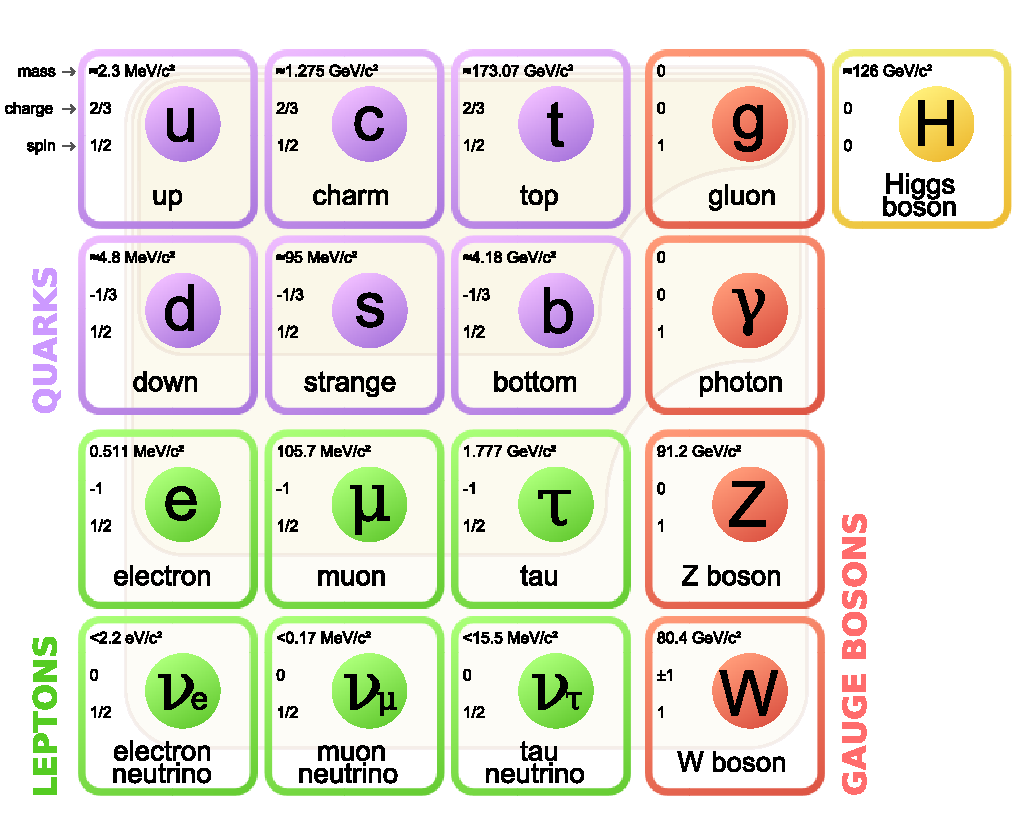
\includegraphics[width=0.85\textwidth]{figs/theory/standardmodel.pdf}
\caption{\label{fig:standardmodel} The particles in the standard model.}
\end{figure}

\begin{table}
\centering
\begin{tabular}{c|ccc}
&$\mathrm{SU(3)}_{\mathrm{C}}$&$\mathrm{SU(2)}_{\mathrm{L}}$&$\mathrm{U(1)}_Y$ \\
$q$ & $\mathbf{3}$ & $\mathbf{2}$ & $1/6$\\
$u^c$ & $\mathbf{\bar 3}$ & $\mathbf{1}$ & $-2/3$\\
$d^c$ & $\mathbf{\bar 3}$ & $\mathbf{1}$ & $1/3$\\
$\ell$ & $\mathbf{1}$ & $\mathbf{2}$ & $-1/2$\\
$e^c$ & $\mathbf{1}$ & $\mathbf{1}$ & $1$\\\hline
$h$ & $\mathbf{1}$ & $\mathbf{2}$ & $1/2$
\end{tabular}
\caption{\label{tab:representations} Table summarizing the
    representations in which the fields transform under the standard
    model gauge group.}
\end{table}


\section{Electroweak symmetry breaking}
The electroweak symmetry $\mathrm{SU(2)}_{\mathrm{L}}\times
\mathrm{U(1)}_Y$ is broken to $\mathrm{U(1)}_{\mathrm{EM}}$.

\section{Higgs mass}


\chapter{Beyond the Standard Model: Theories and Phenomenology}


Supersymmetry.
\section{Coleman-Mandula and $\mathcal{N}=1$ supersymmetry}

As shown by Coleman and Mandula, every local renormalizable quantum
field theory in four-dimensional Minkowski spacetime with
\begin{itemize}
\item finite number of different one-particle states
\item non-trivial interactions
\item mass gap
\end{itemize}
can only have a symmetry \emph{Lie algebra} of the S matrix which is a
direct product of the Poincar\'{e} group and an internal group.

However, this theorem has an infamous loophole in that it assumes the
symmetry algebra of the S matrix contains only commutators, but not
\emph{anticommutators} as a so-called \emph{Lie superalgrebra}
does. In particular, the Lie superalgebra for $\mathcal N=1$
supersymmetry is given in \ref{eqn:n1susy},

\begin{eqnarray}
~\{ Q_{\alpha},\bar Q_{\dot{\beta}}\} &=& 2\sigma^m_{\alpha\dot\beta} P_m \nonumber\\
~\{ Q_{\alpha},Q_{\beta}\} &=& \{ \bar Q_{\dot\alpha},\bar Q_{\dot\beta}\} = 0\nonumber\\
~[ P_m, Q_{\alpha}] &=& [P_m,\bar Q_{\dot\alpha}] = 0
\label{eqn:n1susy}
\end{eqnarray}

\section{Minimal Supersymmetric Standard Model}
The K\"{a}hler potential and super potential for chiral superfields
\begin{equation}
\mathcal L = \int d^4\theta K(\Phi,\Phi^{\dagger}) + \left (\int
  d^2\theta W(\Phi) + \mathrm{h.c.} \right)
\label{eqn:mssmlag}
\end{equation}

\begin{table}
\centering
\begin{tabular}{c|ccc}
&$\mathrm{SU(3)}_{\mathrm{C}}$&$\mathrm{SU(2)}_{\mathrm{L}}$&$\mathrm{U(1)}_Y$ \\
$Q$ & $\mathbf{3}$ & $\mathbf{2}$ & $1/6$\\
$U^c$ & $\mathbf{\bar 3}$ & $\mathbf{1}$ & $-2/3$\\
$D^c$ & $\mathbf{\bar 3}$ & $\mathbf{1}$ & $1/3$\\
$L$ & $\mathbf{1}$ & $\mathbf{2}$ & $-1/2$\\
$E^c$ & $\mathbf{1}$ & $\mathbf{1}$ & $1$\\\hline
$H_u$ & $\mathbf{1}$ & $\mathbf{2}$ & $1/2$\\
$H_d$ & $\mathbf{1}$ & $\mathbf{2}$ & $-1/2$
\end{tabular}
\caption{\label{tab:representations} Table summarizing the
    representations in which the superfields transform under the standard
    model gauge group.}
\end{table}

The R-parity conserving part of the superpotential is whown in Eqn.~\ref{eqn:Wrpc}
\begin{equation}
W_{\mathrm{RPC}} = - y_u H_u Q U^c + y_dH_d Q D^c + y_e H_d L E^c +
\mu H_uH_d
\label{eqn:Wrpc}
\end{equation}
while the R-partiy violating part is shown in \ref{eqn:Wrpv}
\begin{equation}
W_{\mathrm{RPV}} =\frac{1}{2}\lambda^{ijk}L_iL_jE_k^c +
\lambda^{\prime ijk} L_iQ_jD_k^c + \mu^{\prime i}H_uL_i +
\frac{1}{2}\lambda^{\prime\prime ijk}U_i^cD_j^cD_k^c
\label{eqn:Wrpv}
\end{equation}

\section{Simplified natural SUSY models}
\label{sec:sms}

\begin{figure}[htb!]
\centering
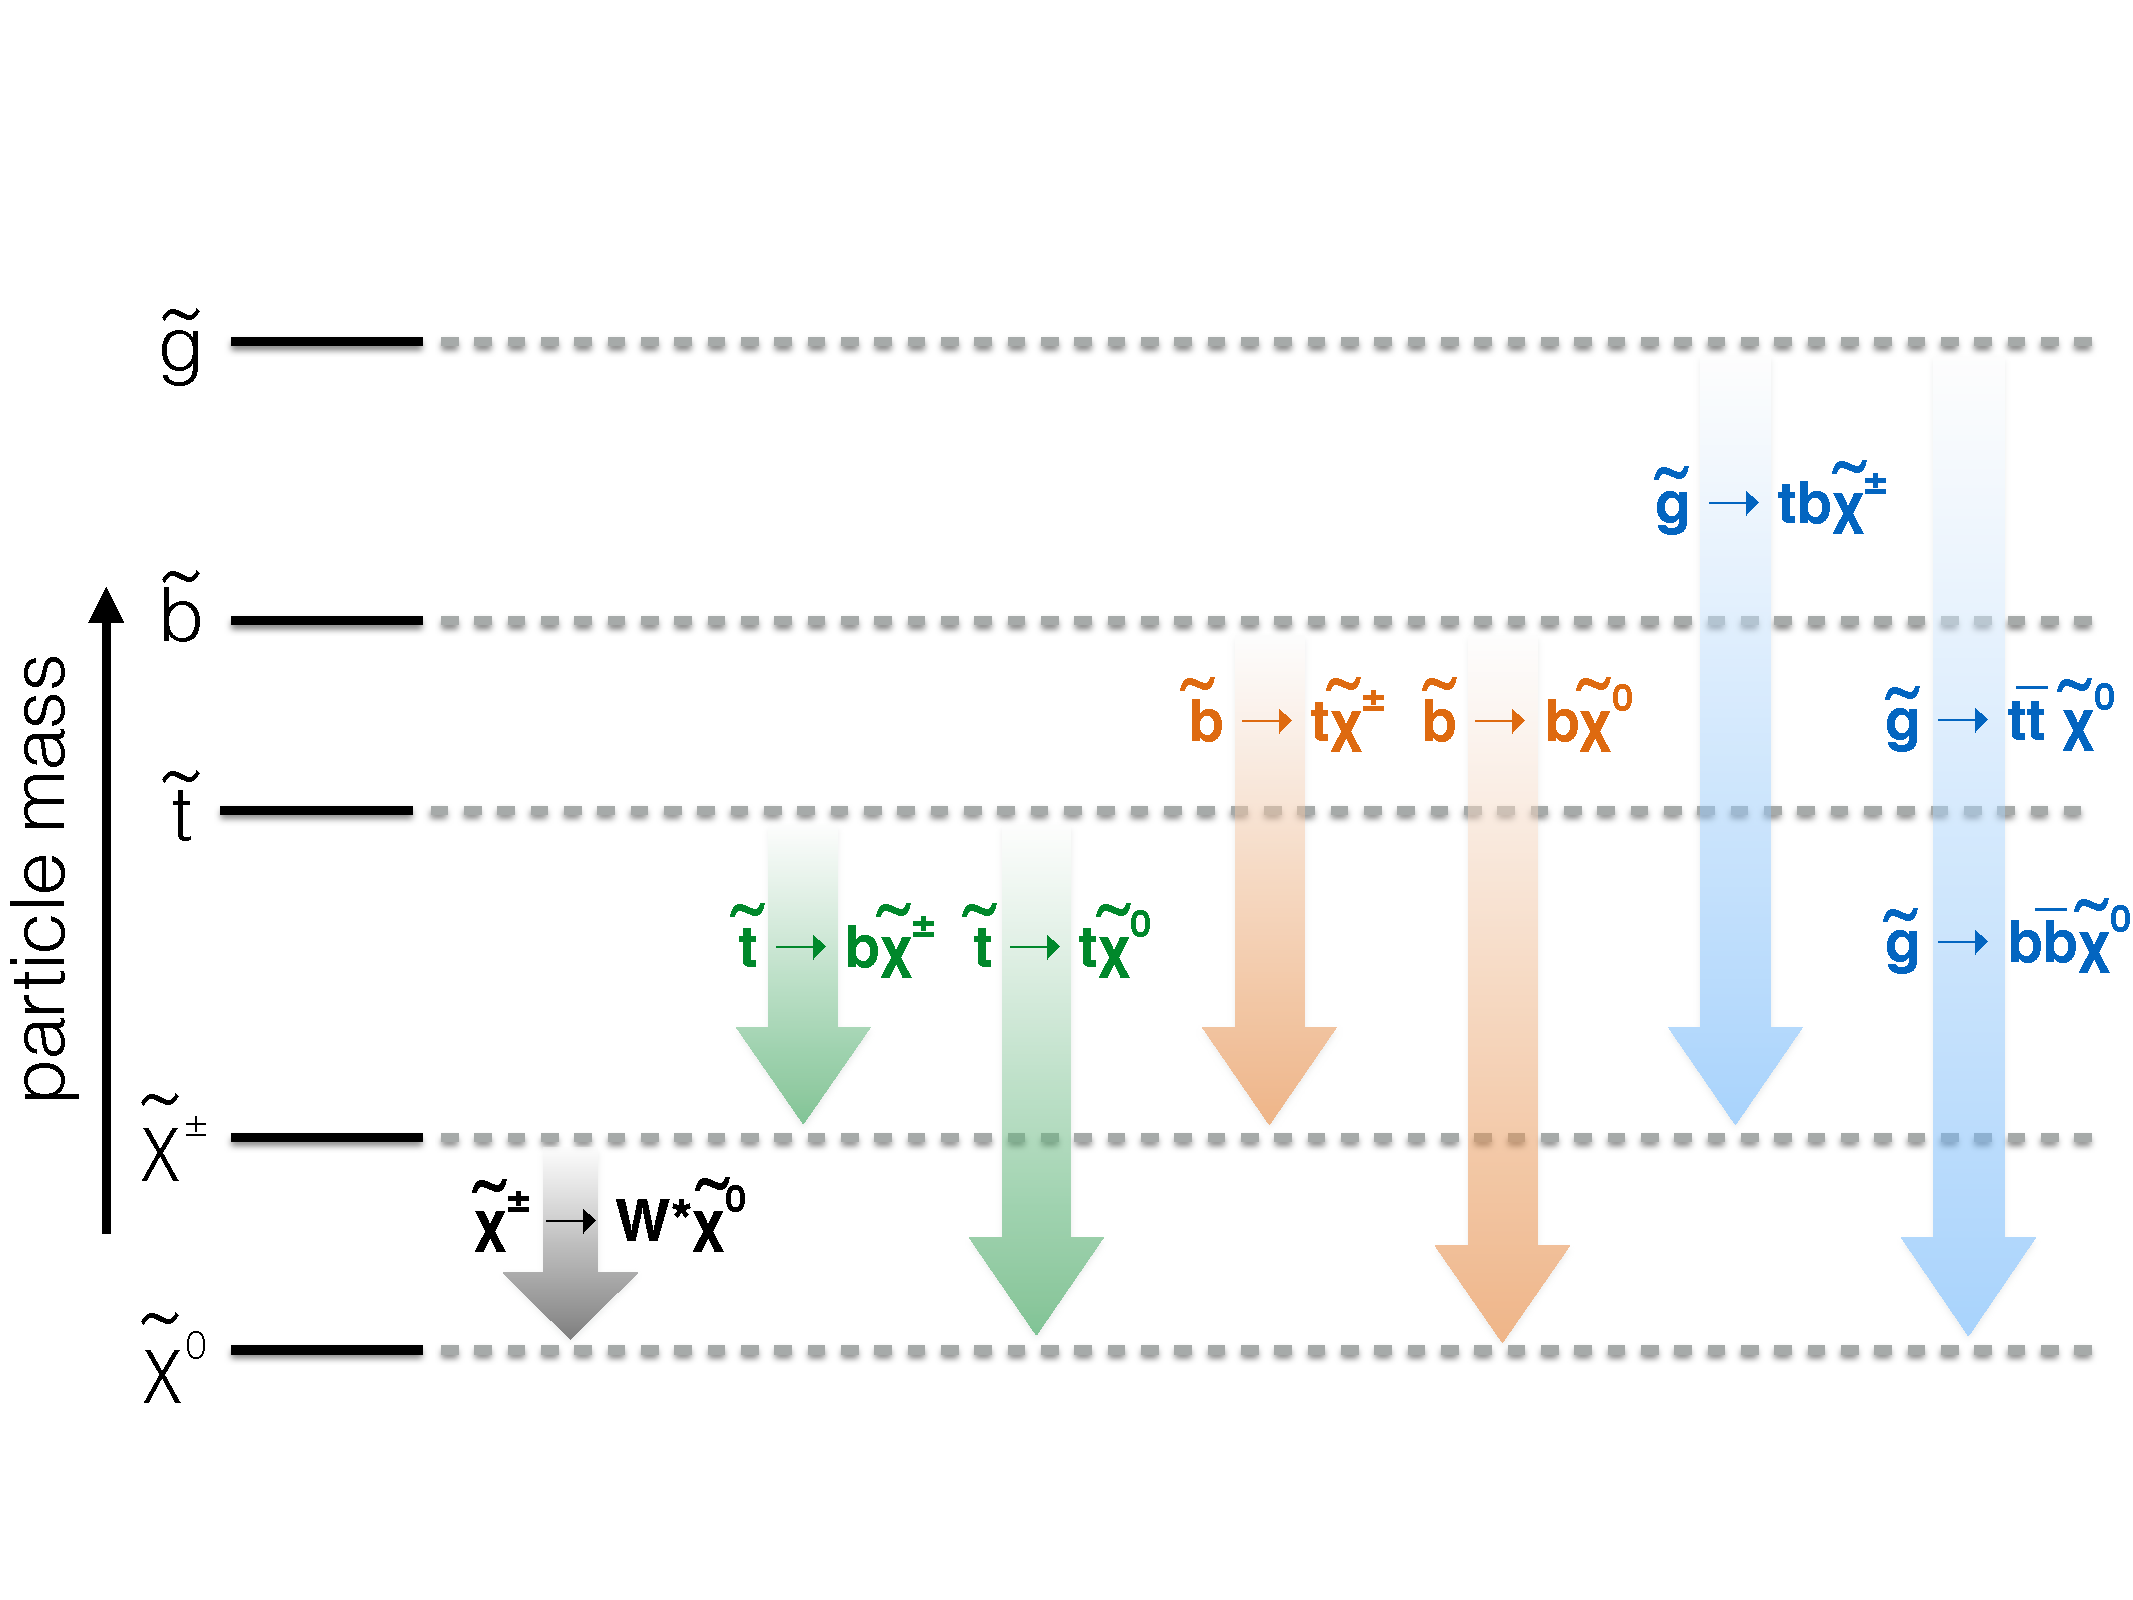
\includegraphics[width=0.85\textwidth]{figs/analysis8TeV/naturalSpectrum.pdf}
\caption{\label{fig:spectrum} The simplified natural SUSY spectrum
  considered in this paper, along with the assumed decay modes.}
\end{figure}

In Chapter~\ref{ch:analysis8TeV}, natural simplified SUSY scenarios are used to interpret
results. The LSP is the lightest neutralino $\chiz_1$ while the NLSP
is the lightest chargino $\chipm_1$.  They are both higgsinos and
their mass splitting is taken to be 5\GeV. The NLSP decays to the LSP
and a virtual $\PW$ boson ($\chipm_1 \to \PW^{\ast} \chiz_1$). The
other SUSY particles accessible at the LHC are the gluino and the
lightest top and bottom squarks. All other SUSY particles are
assumed to be too heavy to participate in the interactions. The SUSY
particles and their possible decay modes within this natural SUSY
spectrum are summarized in Fig.~\ref{fig:spectrum}.

In the context of this natural spectrum, five simplified
models~\cite{ArkaniHamed:2007fw,Alwall:2008ag,Alwall:2008va,Alves:2011sq,Alves:2011wf,Graesser:2012qy}
are considered for gluino pair production, based on three-body gluino decays~\cite{SUS-11-016}:
\begin{itemize}
\item \textbf{ T1bbbb}: pair-produced gluinos, each decaying with a 100\%
 branching fraction to a bottom quark-antiquark ($\bbbar$) pair and the LSP;
\item \textbf{ T1tbbb}: pair-produced gluinos, each decaying with a
 50\% branching fraction to a $\bbbar$ pair and the LSP or to a
 top quark (antiquark), a bottom antiquark (quark), and the NLSP;
\item \textbf{ T1ttbb}: pair-produced gluinos, decaying with a 100\%
  branching fraction to a top quark (antiquark), a bottom antiquark (quark), and the NLSP;
\item \textbf{ T1tttb}: pair-produced gluinos, each decaying with a
 50\% branching fraction to a top quark-antiquark ($\ttbar$) pair and the LSP or to a top
 quark (antiquark), a bottom antiquark (quark), and the NLSP;
\item \textbf{ T1tttt}: pair-produced gluinos, each decaying with a 100\%
 branching fraction to a $\ttbar$ pair and the LSP.
\end{itemize}
The corresponding Feynman diagrams are shown in Fig.~\ref{fig:SMSGluinoTopology}.

\begin{figure*}[thb!]
\centering
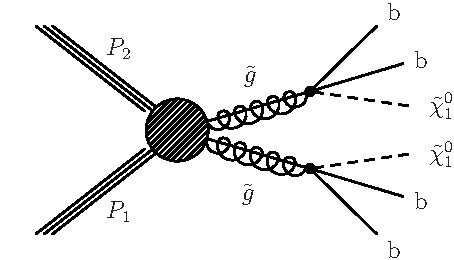
\includegraphics[width=0.32\textwidth]{figs/analysis8TeV/T1bbbb.pdf}
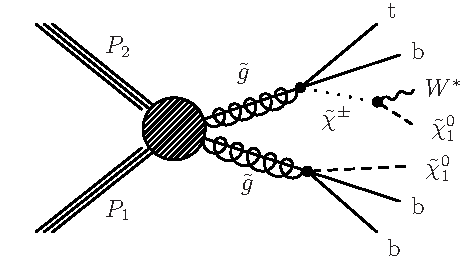
\includegraphics[width=0.32\textwidth]{figs/analysis8TeV/T1tbbb.pdf}
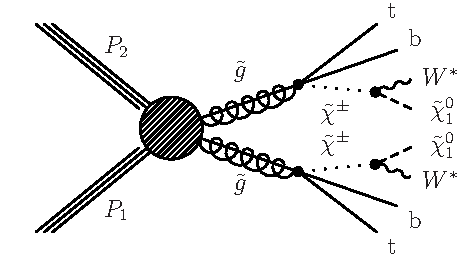
\includegraphics[width=0.32\textwidth]{figs/analysis8TeV/T1ttbb.pdf} \\
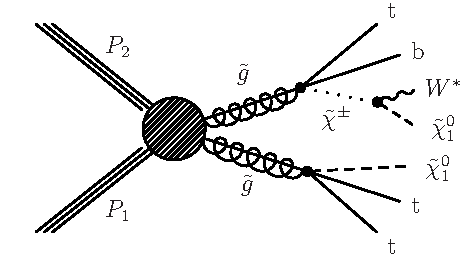
\includegraphics[width=0.32\textwidth]{figs/analysis8TeV/T1tttb.pdf}
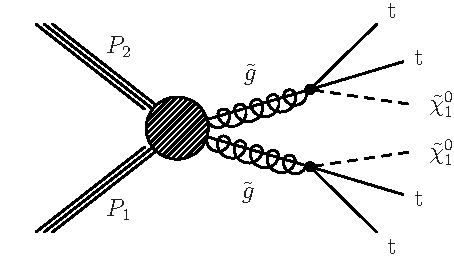
\includegraphics[width=0.32\textwidth]{figs/analysis8TeV/T1tttt.pdf} \\
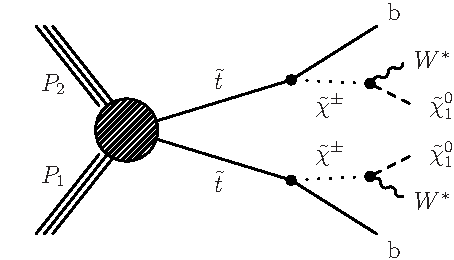
\includegraphics[width=0.32\textwidth]{figs/analysis8TeV/T2bw.pdf}
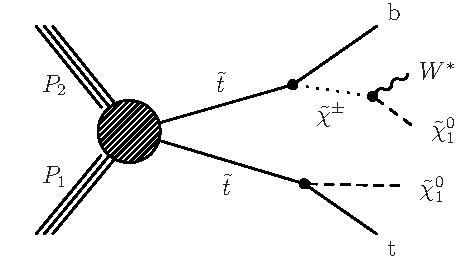
\includegraphics[width=0.32\textwidth]{figs/analysis8TeV/T2tb.pdf}
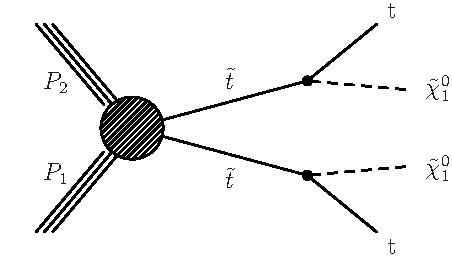
\includegraphics[width=0.32\textwidth]{figs/analysis8TeV/T2tt.pdf}
\caption{Diagrams displaying the event topologies of gluino (upper 5
  diagrams) and top-squark (lower 3 diagrams) pair production
  considered in this paper.\label{fig:SMSGluinoTopology}}
\end{figure*}


In addition, the following three simplified models are considered for
the production of top-squark pairs:
\begin{itemize}
\item \textbf{ T2bW$^{\ast}$}: pair-produced top squarks, each decaying
  with a 100\% branching fraction to a bottom quark and the NLSP;
\item \textbf{ T2tb}: pair-produced top squarks, each decaying with a 50\%
  branching fraction to a top quark and the LSP or to a bottom quark and
  the NLSP;
\item \textbf{ T2tt}: pair-produced top squarks, each decaying with a
  100\% branching fraction to a top quark and the LSP.
\end{itemize}
The corresponding Feynman diagrams are shown in
Fig.~\ref{fig:SMSGluinoTopology}.

\subsection{Technical Implentation in \PYTHIA}
To simplify the treatment of the sparticle decays in \PYTHIA v6.4.26, we directly implement three-body decays of
the form $\chipm_1 \to \chiz_1 f f^{\prime}$, with branching ratios
as shown in Table~\ref{tab:nlspbr}.
\begin{table}
\centering
\begin{tabular}{l|r}
decay mode & branching ratio \\\hline
$\chipm_1 \to \chiz_1 u \bar d$ &  35.1\%\\
$\chipm_1 \to \chiz_1 c \bar s$ &  35.1\%\\
$\chipm_1 \to \chiz_1 e^+ \nu_e$ &  11.7\%\\
$\chipm_1 \to \chiz_1 \mu^+ \nu_{\mu}$ &  11.7\%\\
$\chipm_1 \to \chiz_1 \tau^+ \nu_{\tau}$ &  6.4\%
\end{tabular}
\caption{\label{tab:nlspbr}Table of branching ratios implemented in
  \PYTHIA v6.4.26 for the NLSP
  $\chipm_1$ in the simplified natural SUSY model considered in this chapter.}
\end{table}